\documentclass[a4paper,11.5pt,table]{article}
\usepackage[textwidth=170mm, textheight=230mm, inner=20mm, top=20mm, bottom=30mm]{geometry}
\usepackage[normalem]{ulem}
\usepackage[utf8]{inputenc}
\usepackage[T1]{fontenc}
\PassOptionsToPackage{defaults=hu-min}{magyar.ldf}
\usepackage[magyar]{babel}
\usepackage{amsmath, amsthm,amssymb, paralist, tikz, multirow}
\usetikzlibrary{arrows, positioning}

\usepackage{listings}
\lstset{
	language=C++, 
	basicstyle=\ttfamily, 
	keywordstyle=\color{blue}\ttfamily, 
	stringstyle=\color{red}\ttfamily,
	tabsize = 4
}

\usepackage{hyperref}

\begin{document}
	%%%%%%%%%%%RÖVIDÍTÉSEK%%%%%%%%%%
	\setlength\parindent{0pt}
	\def\<{<\hspace{0mm}<}
	
	\theoremstyle{definition}
	\newtheorem{note}{Megjegyzés}[subsection]
	%%%%%%%%%%%%%%%%%%%%%%%%%%%%%%%%%%%%%%%%%%%%%%%%%%%%%%%%%%%%%%%%%%%%%
	
	\begin{center}
		{\LARGE\textbf{C++}}
		
		{\Large Gyakorlat jegyzet}
		
		5. óra.
	\end{center}
	A jegyzetet \textsc{Umann} Kristóf készítette \textsc{Horváth} Gábor  előadásán. (\today)
	\section{A C++ memóriamodellje}
	A C++ szabvány több memóriatípust különít el. Ezek közül főleg a stack-et használtuk eddig.
	\begin{center}
		\begin{tabular}{|c|}
			\\
			\\
			\\
			\\
			Stack\\
			\\
			\hline
		\end{tabular}\quad 
		\begin{tabular}{|c|}
			\hline
			\quad \quad \\
			\\
			Globális/Statikus\\
			\\
			\hline
		\end{tabular}\quad 
		\begin{tabular}{|c|}
			\hline
			\quad \quad \\
			\\
			Heap/Free store\\
			\\
			\hline
		\end{tabular}
	\end{center}
	\subsection{Stack}
	A második gyakorlaton már volt szó részletesebben a stack működéséről. Jusson eszünkbe egy nagyon fontos tulajdonsága: a blockok végén a változók automatikusan megsemmisülnek. Ebben az esetben nem a programozó feladata a memória felszabadítása.
	\smallskip
	
	A stack-en létrehozott változókat szokás \textbf{automatikus változók}nak (\textit{automatic variable}) is hívni.
	
	\smallskip
	Tekintsük a második gyakorlatról már ismerős kódrészletet.
	
	\begin{lstlisting}
#include <iostream>

int f()
{
	int x = 0;
	++x;
	return x;
}

int main()
{
  for(int i = 0; i < 5; ++i)
	  std::cout << f() << std::endl;
}
	\end{lstlisting}
	Kimenet: \texttt{1 1 1 1 1}
	\smallskip
	
  A stacken lérehozott változók kezelése nagyon kényelmes, mert jól látható, mikor jönnek jönnek létre, mikor semmisülnek meg. Azonban előfordulhat, hogy nem szeretnénk, hogy az \texttt{x} változó élettartama megszűnjön a block végén. Ilyenkor egy lehetőség a statikus változók használata.
	\subsection{Globális/statikus tárhely}
	Írjuk át a fenti \texttt{f} függvényt, hogy \texttt{x} ne automatikus, hanem \textbf{statikus változó} (\textit{static variable}) legyen!
	\begin{lstlisting}
int f()
{
	static int x = 0;
	++x;
	return x;
}

int main() {/*...*/}
	\end{lstlisting}
	Kimenet: \texttt{1 2 3 4 5}
	
  Ebben az esetben azonban a függvény első hivásától a program futásának végéig benne marad a memóriában az \texttt{x}, így mindig egyre nagyobb számokat ad majd \texttt{f()} vissza. Az \texttt{x} inicializációja egyszer történik meg, a függvény első hívásakor. 
	\begin{note}
		Nem szeretjük a \texttt{static} változókat. Például a több szálú programok esetén különösen kerülendő ez a programozási stílus.
	\end{note}

  A globális változók és a statikus változók a memória ugyanazon területén jönnek létre. Ezért hívjuk ezt a területet globális/statikus tárhelynek.

  \medskip
	Amennyiben azt szeretnénk, hogy \texttt{x} ne semmisüljön meg a block végén, de ne is maradjon a program futásának a végéig a memóriában, arra is van lehetőség. Ebben az esetben viszont a programozó felel a memória kezeléséért.
	\subsection{Heap/Free store}
	A heapen létrehzoott változókat \textbf{dinamikus változók}nak (\textit{dynamic variable}) is szokás szokás hívni. A heap segítségével nagy szabadságra tehetünk szert, azonban ez a szabadság nagy felelősséggel is jár.
	\begin{lstlisting}
int main()
{
	int *p = new int(2);
	delete p;
}
	\end{lstlisting}
	Fentebb láthatjuk hogyan lehet egy intnek lefoglalni helyet a heapen. Fontos, hogy a stack-et nem kerültük meg, mert szükségünk van egy pointerre, mely a heap-en lefoglalt címre mutat (\texttt{p}).
	
	A mutató által mutatott területet a \texttt{delete} operátorral tudjuk felszabadítani.
	\begin{figure}[!h]
		\centering
		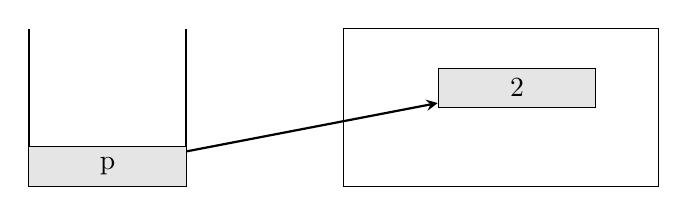
\begin{tikzpicture}
		\tikzstyle{Heap} = [rectangle, minimum width=4cm, minimum height=2cm, text centered, draw=black, fill=white]
		\tikzstyle{Stack} = [rectangle, minimum width=3cm, minimum height=1cm, text centered, draw=black, fill=white]
		\tikzstyle{ListNode} = [rectangle, minimum width=2cm, minimum height=5mm, text centered, draw=black, fill= gray!20]
		\tikzstyle{arrow} = [thick,->,>=stealth]
		
		%\foreach \x in {-2,-1,0,1,2,3,4}
		%	\draw (\x cm,1pt) -- (\x cm,-1pt) node[anchor=north] {$\x$};
		%\foreach \y in {-2,-1,0,1,2,3,4}
		%	\draw (1pt,\y cm) -- (-1pt,\y cm) node[anchor=east] {$\y$};
		%\draw[step=5mm,gray,very thin] (-2,-2) grid (6,6);
		
		\draw [thick, black] (-3, 0) -- (-1, 0);
		\draw [thick, black] (-3, 0) -- (-3, 2);
		\draw [thick, black] (-1, 0) -- (-1, 2);
		\node[Heap] at (3,1){};
		\node (2) [ListNode] at (3.2,1.25) {2};
		\node (p) [ListNode] at (-2,0.25) {p};
		\draw[arrow] (p) -- (2);
		\end{tikzpicture}
	\end{figure}
	
	A heapen nincs a lefoglalt területnek nevük, így mindig szükségünk lesz egy mutatóra, hogy tudjunk rá hivatkozni. \textbf{Ha egyszer lefoglalunk valamit a heap-en, gondoskodni kell arról, hogy felszabadítsuk.} Az egyik leggyakoribb hiba a dinamikus memóriakezelésnél, ha a memóriát nem szabadítjuk fel. Ilyenkor a lefoglalt memóriaterületre hivatkozni már nem tudunk de lefoglalva marad: elszivárog (\textit{memory leak}). 
	\smallskip
	
	Bár az operációs rendszer megpróbál minden, a program által lefoglalt memóriát felszabadítani a futás befejeztével, de nem mindenható. Előfordulhat, hogy egyes platformokon újraindításig nem szabadul fel a memória. Emellett ameddig a program fut, több memóriát fog használni, mint amennyire szüksége van. Ez növelheti a szerverpark költségeit vagy ronthatja a felhasználói élményt.
	\medskip
	
	A dinamikusan lefoglalt memória szabályos felszabadítását számos dolog nehezíti. Fényes példa erre a kivételkezelés, melynél hamarabb megszakadhat a függvény végrehajtása mintsem, hogy felszabadítson minden memóriát. Előfordulhat, hogy egy memóriaterületet kétszer szabadítunk fel, ami nem definiált viselkedés.
	\medskip
	
  Előfordulhat, hogy egy már felszabadított memóriaterületre akarunk írni vagy onnan olvasni. Sajnos ilyen jellegű hibát könnyű véteni, hisz a \texttt{delete} a \texttt{p} által mutatott memóriaterületet, nem a \texttt{p}-t fogja törölni. A \texttt{p} továbbra is használható.
	\begin{note}
		A nullpointer törlésekor nem történik semmi (\textit{no-op}).
	\end{note}
	\begin{note}
		Amint elvesztettük az utolsó mutatót, ami egy adott lefoglalt memóriacímre mutat, az garantáltan elszivárgott memória. A szabvány nem foglal magában semmilyen lehetőséget ezeknek a visszaszerzésére.
	\end{note}
	Láthatjuk, hogy a heap használata hibalehetőségekkel teli, ráadásul az allokálás (memória lefoglalás) még lassabb is, mintha a stack-et használnánk. De miért használjuk mégis? Ha meg lehet oldani, hogy a stack-en tudjunk tárolni valamit, tegyük azt. A stacken azonban véges, hamar be tud telni (\textit{stack overflow}), illetve kötött a változók élettartama. A heap-en e téren sokkal nagyobb a szabadságunk.
	\section{Osztályok felépítése}
	A következő pár gyakorlaton egy láncolt listát fogunk implementálni, mely jól demonstrálja majd a dinamikus memóriakezelés veszélyeit is.
	
	\smallskip
	A láncolt lista egy olyan konténer, melynek minden eleme egy olyan listaelem, mely tartalmaz egy mutatót és (legalább egy) adatot tároló objektumot. A listaelem mutatója rámutat a lista következő elemére, és az utolsó elem pointere pedig egy nullpointer.
	\begin{center}
		\begin{tabular}{|c|c|}
			\hline
			\texttt{data}&\texttt{*next}\\
			\hline
		\end{tabular}
		\smallskip
		
		Egy listaelem.
		\medskip
		
		\begin{tabular}{|c|c|}
			\hline
			\texttt{8}&\texttt{}\\
			\hline
		\end{tabular}$\rightarrow$
		\begin{tabular}{|c|c|}
			\hline
			\texttt{7}&\texttt{}\\
			\hline
		\end{tabular}$\rightarrow$
		\begin{tabular}{|c|c|}
			\hline
			\texttt{2}&\texttt{$\emptyset$}\\
			\hline
		\end{tabular}
		\smallskip
		
		3 elemű láncolt lista.
	\end{center}
	\subsection{Struct-ok}
	Egy láncolt lista elemét implementálhatjuk pl. így:
	\begin{lstlisting}
struct List
{
	int data;
	List *next;
};
	\end{lstlisting}
	Alkalmazzuk is ezt úgy, hogy  a listaelemek dinamikusan legyen eltárolva!
	\begin{lstlisting}
int main()
{
	List *head = new List;
	head->data = 8; //(*head).data   ==   head->data
	head->next = new List;
	
	head->next->data = 7;
	head->next->next = new List;
	
	head->next->next->data = 2;
	head->next->next->next = NULL;
	
	delete head;
	delete head->next;
	delete head->next->next;
}
	\end{lstlisting}
	Ezen a ponton készen vagyunk, hisz \texttt{List} használható láncolt listaként (bár valójában igen kényelmetlen).
	\medskip
	
	\begin{figure}[!h]
		\centering
		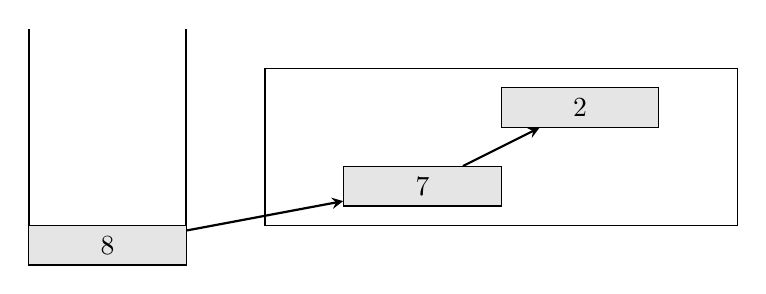
\begin{tikzpicture}
		\tikzstyle{Heap} = [rectangle, minimum width=6cm, minimum height=2cm, text centered, draw=black, fill=white]
		\tikzstyle{Stack} = [rectangle, minimum width=3cm, minimum height=1cm, text centered, draw=black, fill=white]
		\tikzstyle{ListNode} = [rectangle, minimum width=2cm, minimum height=5mm, text centered, draw=black, fill= gray!20]
		\tikzstyle{arrow} = [thick,->,>=stealth]
		
		%\foreach \x in {-2,-1,0,1,2,3,4}
		%	\draw (\x cm,1pt) -- (\x cm,-1pt) node[anchor=north] {$\x$};
		%\foreach \y in {-2,-1,0,1,2,3,4}
		%	\draw (1pt,\y cm) -- (-1pt,\y cm) node[anchor=east] {$\y$};
		%\draw[step=5mm,gray,very thin] (-2,-2) grid (6,6);
		
		\draw [thick, black] (-3, 0) -- (-1, 0);
		\draw [thick, black] (-3, 0) -- (-3, 3);
		\draw [thick, black] (-1, 0) -- (-1, 3);
		\node[Heap] at (3,1.5){};
		\node (7node) [ListNode] at (2,1) {7};
		\node (2node) [ListNode] at (4,2) {2};
		\node (headNode) [ListNode] at (-2,0.25) {8};
		\draw [arrow] (7node) -- (2node);
		\draw [arrow] (headNode) -- (7node);
		\end{tikzpicture}
	\end{figure}
	Sajnos a törlést rossz: először törljük a fejelemet (mely az első elemre mutat), viszont az első elem segítségével tudnánk a többi elemet elérni, így mikor a második listaelemet törölnénk, \texttt{head} már egy felszabadított memóriaterületre mutat. Ezt törlés utáni használatnak (\textit{use after delete}) szokás nevezni és nem definiált viselkedés.
	
	A megoldás:
	\begin{lstlisting}
delete head->next->next;
delete head->next;
delete head;
	\end{lstlisting}
	\begin{note}
		A heap-en arra is figyelni kell, hogy jó sorrendben szabadítsuk fel a memóriát. Ha rossz sorrendben szabadítjuk fel az objektumokat, könnyen a fentihez hasonló hibát vagy memória szívárgást okozhatunk.
	\end{note}
	A változók a stacken a létrehozás sorrendjéhez képest fordított sorrendben semmisülnek meg, pont emiatt.
	\medskip
	
	Ez a ,,láncolt lista'' eddig elég szegényes. A fő gond az, hogy nagyon sokat kell írni a használatához. Ez sért egy programozási elvet, a DRY-t : \textit{Dont Repeat Yourself}. Itt sokszor írjuk le közel ugyanazt -- erre kell, hogy legyen egy egyszerűbb megoldás. Írjunk függvényt az új listaelem létrehozásához!
	\begin{lstlisting}
List *add(List *head, int data)
{
	if (head == 0)
	{
		List *ret = new List;
		ret->data = data;
		ret->next = 0;
		return ret;
	}
	head->next = add(head->next, data);
	return head;
}
	\end{lstlisting}
	Ez egy olyan rekurzív függvény, mely addig hívja saját magát, míg a paraméterként kapott lista végére nem ér (azaz a \texttt{head} egy nullpointer). Amikor oda elér, létrehoz egy új listaelemet és azt visszaadja. A rekurzió felszálló ágában a lista megfelelő elemeit összekapcsolja. 
	\medskip
	
	Írjunk egy függvényt a lista által birtokolt memória felszabadítására is.
	\begin{lstlisting}
void free(List *head)
{
	if (head == 0)
		return;
	free(head->next);
	delete head;
}
	\end{lstlisting}
	Itt a rekurzió szintén a lista végéig megy. A rekurzió felszálló ágában történik a listaelemek felszabadítása. Ennek az oka, hogy a felszabadítás a megfelelő sorrendben történjen meg.
	\begin{note}
		A rekurzív függvények nem olyan hatékonyak, mint az iterativ (pl. \texttt{for} vagy \texttt{while} ciklus) társaik. Továbbá a sok függvényhívás könnyen stack overflow-hoz vezetnek. Azonban jó agytornák, és segíthetnek az alapötletben. Egy rekurzív függvényt mindig át lehet írni iteratívvá.
	\end{note}
	Beszéljünk arról, mennyi a teher a felhasználón. Eddig tudnia kellett, milyen sorrendben kell felszabadítani az elemeket a listán belüle, de most már elég arra figylenie, hog lista használata után meghívja a \texttt{free} függvényt. A felhasználó így kisebb eséllyel követ el hibát, több energiája marad arra, hogy az előtte álló problémát megoldja. Legyenek a függvényeink és osztályaink olyanok, hogy \textbf{könnyű legyen őket jól használni, és nehéz legyen rosszul}.
	
	\subsection{Osztályra statikus változók}
	Teszteljünk!
	\begin{lstlisting}
int main()
{
	List *head = 0;
	head = add(head, 8);
	head = add(head, 7);
	head = add(head, 2);
	
	free(head);
}
	\end{lstlisting}
	A program lefordult, és a gyakorlaton tökéletesen le is futott. Azonban, ha történt memory leak vagy double free, esetleg use after free, az nem definiált viselkedés. Ezért nem lehetünk benne biztosak, hogy valóban nem történt memóriakezeléssel kapcsolatos hiba. A sanitizerek segítségével megyőződhetünk róla, hogy nem követtünk el ilyen jellegű hibát.
	
	\smallskip
	Az osztályon belül statikusként deklarált változókat osztályszintű változóknak is hívjuk, ugyanis minden, az osztályhoz tartozó objektum ugyanazon a statikus változón ,,osztozkodik''. Ha az egyiken keresztül azt a változót módosítjuk, a többiben módosulni fog. Élettartamuk és láthatóságuk a program elejétől végéig tart.
	
	Hozzunk létre \texttt{List}-ben egy számlálót, ami számon tartja mennyi objektumot hoztunk belőle létre, és semmisítettünk meg! Ezzek a trükkel megnézhetjük, hogy elfelejtettünk-e felszabadítani listaelemet.
	\begin{lstlisting}
struct List
{
	int data;
	List *next;
	
	static int count; // !
};

int List::count = 0;

List *add(List *head, int data)
{
	if (head == 0)
	{
		List *ret = new List;
	    List::count++; // !
		ret->data = data;
		ret->next = 0;
		return ret;
	}
	head->next = add(head->next, data);
	return head;
}

void free(List *head)
{
	if (head == 0)
	return;
	free(head->next);
	List::count--; // !
	delete head;
}

int main()
{
	List *head = 0;
	head = add(head, 8);
	head = add(head, 7);
	head = add(head, 2);
	
	free(head);
	std::cout << List::count; // !
}
	\end{lstlisting}
	
	Osztályszintű változókat csak osztályon kívül tudunk definiálni (ezek alól kivételt képeznek az osztályszintű konstans változók), ezért látható az osztály után a következő sor:
	\begin{lstlisting}
int List::count = 0;
	\end{lstlisting}
	
	Ezzel a kis módosítással meg is kapjuk a kívánt kimenetet: \texttt{0}. Ez alapján tudhatjuk, hogy minden objektum törlésre került.
	\begin{note}
		A fenti módosítások csak gyakorlás célját képezték, az elkészítedő listának nem része a számláló.
	\end{note}
	Ha azonban egy elemet kétszer töröltünk, egyet meg elszivárogtattunk, az nem feltétlen nem derül ki. Ilyenkos a sanitizerek segíthetnek:
	\begin{center}
		\texttt{g++ list.cpp -fsanitize=address -g}
	\end{center}
  A sanitizerekről bővebben lásd a 3. gyakorlat anyagát.
	\medskip
	Határozott előrelépést értünk el, de van még hova fejleszteni a listánkat. Szerencsére nem csak adattagokat, de tagfüggvényeket is tudunk struct-okba írni.
	\subsection{Konstruktorok}
	Egy trükkel megoldható, hogy tömörebb szintaxissal tudjuk inicializálni a listaelemeinket.
	\begin{lstlisting}
struct List
{
	List(int _data, List *_next = 0) : data(_data), next(_next) {}
	
	int data;
	List *next;
};
	\end{lstlisting}
	A fenti tagfüggvényt, vagy metódust \textbf{konstruktor}nak (\textit{constructor}, vagy röviden \textit{ctor}) hívjuk. A konstruktorok hozzák létre az objektumokat; vannak paraméterei, és nincs visszatérési értéke. A fenti konrtruktor még egy alapértelmezett paraméterrel is rendelkezik - ha mi csak egy \texttt{int} paraméterrel hívjuk meg a konstruktort, akkor a \texttt{\_next}-et alapértelmezetten nullpointernek veszi.
	
	\medskip
	Azonban a struktúránk működött eddig is, pedig nem írtunk konstruktort. Ha konstruktorra szükség van objektum létrehozáshoz, akkor hogyan lehet ez? Úgy, hogy a fordító a hiányzó kulcsfontosságú függvényeket legenerálja nekünk. Létrehoz (többek között) egy un. \textbf{default konstruktort}, ha mi explicit nem hoztunk létre konstruktort. A default konstruktor 0 paraméterrel meghívható. Fontos azonban, ha mi írunk egy konstruktort, akkor a fordító már nem fog generálni ilyet.
	
	\medskip
	A konstruktor fejléce után található egy un. \textbf{inicializációs lista}. Az inicializációs lista hasonló jelentéssel bír, mint a következő kód:
	\begin{lstlisting}
List(int _data, List *_next = 0)
{
	data = _data;
	next = _next;
}
	\end{lstlisting}
  Az inicializációs lista használata azonban hatékonyabb.
	Mire a konstruktor törzséhez érünk, addigra az adattagoknak inicializálva kell lenniük. A trözsben ezért már inicializált értékeket írunk felül, ami erőforráspazarlás. Primitív típusok esetén ez nem jelent problémát, összetett típusok esetén viszont számottevő lehet.
	\begin{note}
    A konstruktor törzsében történő értékadás 2 lépés (mivel előtte egy alapértelmezett konstruktor már inicializálta az objektumot), az inicializálás csak 1.
	\end{note}
	Fontos megjegyzés, hogy az a struktúra elemei a meződ definiálásának a sorrendjében inicializálódnak. Tehát, bármilyen sorrendben írjuk mi az inicializációs listát, mindig először a \texttt{data}, és utána a \texttt{next} fog inicializálódni.
	\subsection{Destrukorok}
	Ahogy gondoskodtunk a listaelemek létrehozásáról, gondoskodhatnánk annak megfelelő megsemmisüléséről is.
	\begin{lstlisting}
struct List
{
	List(int data, List *next = 0) : data(data), next(next) {}
	~List() // dtor
	{
		delete next;
	}
	
	int data;
	List *next;
};
	\end{lstlisting}
	Az fenti tagfüggvényt, melynél a hullámvonalat közvetlenül a struktúra neve követi \textbf{destruktor}nak (\textit{destruktor}, röviden \textit{dtor}) nevezzük. A destruktor mindig az objektum élettartamának végén hívódik meg, és gondoskodik a megfelelő erőforrások felszabadításáról. 
	
	\medskip
	A destruktort is rekurzívan írtuk meg: a \textbf{next} által mutatott memóriaterület felszabadításakor meghívja \texttt{List} típusú elem destruktorát. A lista végén a \texttt{next} egy nullpointer, azon a delete hívás nem csinál semmit.
	
	\medskip
	Teszteljünk!
	\begin{lstlisting}
int main()
{
	List head(8);
	add(&head, 7);
	add(&head, 2);
}
	\end{lstlisting}
	Most úgy alakítottuk át a kódot, hogy amikor létrehozzuk a listát, akkor a fejelemet a stacken hozzuk létre, melynek értéke 8, és a pointer része nullpointer. Később az \texttt{add} függvénnyel létrehozunk a heapen egy olyan listaelemet, mely 7-et tárol, és pointer része nullpointer, és az eredeti lista fejét ráállítjuk erre.
	\medskip
	
	Itt sikeresen elértük, hogy a lista első eleme a stack-en, de minden más eleme a heap-en legyen. Mivel olyan struktrát írtunk, mely gondoskodik arról, hogy minden dinamikusan lefoglalt területet felszabadítson, mindent csak egyszer töröl, jó sorrendben, egy  \textit{RAII} (\textit{Resource acquisition is initialization}) osztályt írtunk. Ez Bjarne-nek egy elég szerencsétlenül választott acronymje. A lényege, hogy az adott osztály a megfelelő erőforrásokat lefoglalja magának, majd a destruktor gondoskodik az erőforrások felszabadításáról. Minden erőforrást egy stack-en lévő objektumhoz kötünk, mivel azok garantáltan automatikusan fel fognak szabadulni, a destruktoruk le fog futni. Jelen esetben a lista fejeleme, ami a stack-en van, felelős azért, hogy a heap-re allokált listaelemek felszabaduljanak a program futásának a végeztével. Így a felhasználónak már a free hívásra sem kell figyelnie.
	
	Bjarne híres mondása, hogy a C++ szemétgyüjtéssel rendelkező nyelv, mert nem generál szemetet. A jól megírt objektumok mindig eltakarítanak maguk után. 
	\medskip
	
	A konstruktor/destruktor használata ugyanolyan hatékony, mintha kézzel kezeltük volna a memóriát.
	
	\medskip
	Csináljunk az \texttt{add} függvényből tagfüggvényt!
	\begin{lstlisting}
struct List
{
  // ...	
	void add(int data) //eltunt egy parameter!
	{
		if (next == 0)
		{
			next = new List(data);
		}
		else
		{
			next->add(data);
		}
	}
	int data;
	List *next;
};

int main()
{
	List head(8);
	head.add(7);
	head.add(2);
}
	\end{lstlisting}
	A nyelv egyik szépsége, hogy a felhasználónak nem kell tudnia, hogy hogyan reprezentáltuk a listát. A listát az a felhasználó is tudja használni, aki nem ismeri a heap-et, nem hallott még soha láncolt adatszerkezetekről. A későbbiekben a lista prerezentációja kicserélhető akár egy vektor szerű adatszerkezetre anélkül, hogy a felhasználói kódot módosítani kellene.
	\medskip
	
	\subsection{Másoló konstruktor}
	
	A fordító sok kódot generál a structunkba: konstruktoron és destruktoron kívül még \textbf{másoló konstruktor}t (\textit{copy constructor}) is. A másoló konstruktor egy olyan konstrukor, melynek egyetlen paramétere egy azonos típusú objektum. Ez alapértelmezetten minden adattagot lemásol az adott adattag másoló konstruktora segítségével. Primitív típusoknál ez bitről bitre másolást jelent. Mi ennek a következménye?
	\begin{lstlisting}
int main()
{
	List head(8);
	head.add(7);
	head.add(2);
	{
		List cHead = head;
	} //itt lefut cHead destruktora
}
	\end{lstlisting}
	Fentebb létrehoztunk egy új listát \texttt{head} mintájára. A másolatnak a destruktora hamarabb lefut. Ha sanitizerrel fordítunk, futáskor hibaüzenetet kapunk: felszabadított memóriaterületet szeretnénk használni. Ennek az az oka, hogy a \texttt{cHead}-ben lévő pointer \textbf{ugyanarra} a listára fog mutatni (lévén a bitről bitre történő másolás történt a pointernél). A \texttt{cHead} megsemmisülése után a \texttt{head} destruktora megpróbál beleolvasni a már felszabadított memóriaterületbe.
	
	%\resizebox{\textwidth}{!}{%
	\begin{figure}[!h]
		\centering
		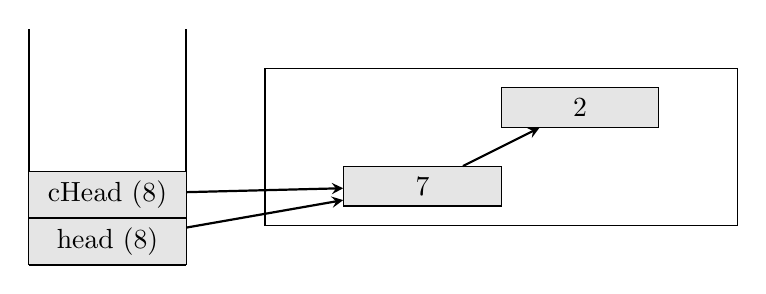
\begin{tikzpicture}
			\tikzstyle{Heap} = [rectangle, minimum width=6cm, minimum height=2cm, text centered, draw=black, fill=white]
			\tikzstyle{Stack} = [rectangle, minimum width=3cm, minimum height=1cm, text centered, draw=black, fill=white]
			\tikzstyle{ListNode} = [rectangle, minimum width=2cm, minimum height=5mm, text centered, draw=black, fill= gray!20]
			\tikzstyle{arrow} = [thick,->,>=stealth]
			
			%\foreach \x in {-2,-1,0,1,2,3,4}
			%	\draw (\x cm,1pt) -- (\x cm,-1pt) node[anchor=north] {$\x$};
			%\foreach \y in {-2,-1,0,1,2,3,4}
			%	\draw (1pt,\y cm) -- (-1pt,\y cm) node[anchor=east] {$\y$};
			%\draw[step=5mm,gray,very thin] (-2,-2) grid (6,6);
			
			\draw [thick, black] (-3, 0) -- (-1, 0);
			\draw [thick, black] (-3, 0) -- (-3, 3);
			\draw [thick, black] (-1, 0) -- (-1, 3);
			\node[Heap] at (3,1.5){};
			\node (7node) [ListNode] at (2,1) {7};
			\node (2node) [ListNode] at (4,2) {2};
			\node (cHeadNode) [ListNode] at (-2,0.9) {cHead (8)};
			\node (headNode) [ListNode] at (-2,0.3) {head (8)};
			\draw [arrow] (7node) -- (2node);
			\draw [arrow] (headNode) -- (7node);
			\draw [arrow] (cHeadNode) -- (7node);
		\end{tikzpicture}
		\smallskip
		
		Zárójelben a lista első elemének \texttt{data} adattagjának értéke.
	\end{figure}
	%}
	
	A megoldás egy saját másoló konstruktor bevezetése!
	
	
\begin{lstlisting}
struct List
{
	//...
	
	List(const List &other) : data(other.data), next(0)
	{
		if (other.next != 0)
		{
			next = new List(*other.next);
		}
	}
	
	//...
};

int main()
{
	List head(8);
	head.add(7);
	head.add(2);
	{
		List cHead = head;
	}
}
\end{lstlisting}
	Mint a korábbi függvényeink, ez is rekurzív: a \texttt{new List(*other.next)} újra meghívja a copy konstruktort, ha az other.next nem nullpointer.
	\begin{figure}[!h]
		\centering
		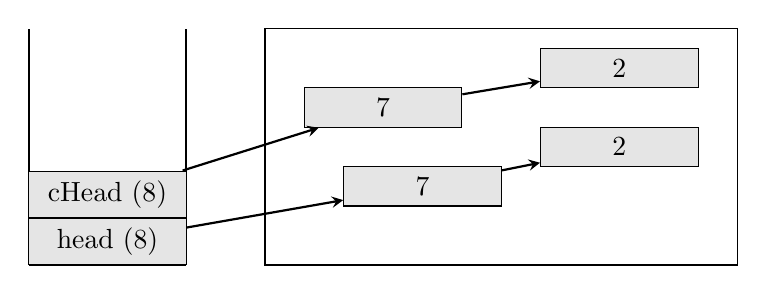
\begin{tikzpicture}
		\tikzstyle{Heap} = [rectangle, minimum width=6cm, minimum height=3cm, text centered, draw=black, fill=white]
		\tikzstyle{Stack} = [rectangle, minimum width=3cm, minimum height=1cm, text centered, draw=black, fill=white]
		\tikzstyle{ListNode} = [rectangle, minimum width=2cm, minimum height=5mm, text centered, draw=black, fill= gray!20]
		\tikzstyle{arrow} = [thick,->,>=stealth]
		
		%\foreach \x in {-2,-1,0,1,2,3,4}
		%	\draw (\x cm,1pt) -- (\x cm,-1pt) node[anchor=north] {$\x$};
		%\foreach \y in {-2,-1,0,1,2,3,4}
		%	\draw (1pt,\y cm) -- (-1pt,\y cm) node[anchor=east] {$\y$};
		%\draw[step=5mm,gray,very thin] (-2,-2) grid (6,6);
		
		\draw [thick, black] (-3, 0) -- (-1, 0);
		\draw [thick, black] (-3, 0) -- (-3, 3);
		\draw [thick, black] (-1, 0) -- (-1, 3);
		\node[Heap] at (3,1.5){};
		\node (7node) [ListNode] at (2,1) {7};
		\node (2node) [ListNode] at (4.5,1.5) {2};
		\node (7node2) [ListNode] at (1.5,2) {7};
		\node (2node2) [ListNode] at (4.5,2.5) {2};
		\node (cHeadNode) [ListNode] at (-2,0.9) {cHead (8)};
		\node (headNode) [ListNode] at (-2,0.3) {head (8)};
		\draw [arrow] (7node) -- (2node);
		\draw [arrow] (7node2) -- (2node2);
		\draw [arrow] (headNode) -- (7node);
		\draw [arrow] (cHeadNode) -- (7node2);
		\end{tikzpicture}
	\end{figure}
	
	\medskip
	Ezzel meg is oldottuk a problémát. 
	
	Figyelem, ez egy \textbf{copy konstruktor, nem értékadás operátor!} Itt a \texttt{cHead} még nincs létrehozva, amikor head-el \textbf{inicializáljuk}. Ha az egyenlőségjel bal oldalán lévő objektum még nem jött létre, mint itt, akor a copy konstruktor hívás történik. Ellenkező esetben értékadás operátor.
	\begin{lstlisting}
List cHead = head; //copy ctor

List cHead;
cHead = head; //ertekadas
	\end{lstlisting}
	
\end{document}
